\documentclass[12pt,a4paper]{report}

% --- Paquetes de Idioma y Codificación ---
\usepackage[utf8]{inputenc}
\usepackage[T1]{fontenc}
\usepackage[english]{babel}

% --- Diseño de Página ---
\usepackage{geometry}
\geometry{top=2.5cm, bottom=2.5cm, left=3cm, right=3cm}

% --- Matemáticas y Símbolos ---
\usepackage{amsmath, amssymb, amsthm}
\usepackage{cancel}

% --- Colores y Cajas ---
\usepackage[dvipsnames]{xcolor}
\usepackage[most]{tcolorbox}

% Caption

\usepackage{caption}

% Gráficos

\usepackage{graphicx}

% Espaciadora

\newcommand{\esp}{\vspace{0.5cm}}

% promedio

\newcommand{\prom}[1]{\left\langle #1 \right\rangle}

% Bibliografía

\usepackage[style=apa, backend=biber]{biblatex} % Estilo APA
\addbibresource{biblio.bib} % Nombre de tu archivo .bib

% Configuración de cajas personalizadas
\newtcolorbox{importante}{
	colback=red!5!white,
	colframe=red!75!black,
	title=Importante,
	fonttitle=\bfseries
}

\newtcolorbox{nota}{
	colback=blue!5!white,
	colframe=blue!75!black,
	title=Nota,
	fonttitle=\bfseries
}

% Definición de la caja de bibliografía
\newtcolorbox{bibliografia}{
	colback=gray!5!white,
	colframe=gray!75!black,
	title=Bibliografías útiles,
	fonttitle=\bfseries,
	breakable
}

% Socrative para óptica 2

\newtcolorbox{Socrative}{
	colback=orange!5!white,
	colframe=orange!75!black,
	title=Socrative,
	fonttitle=\bfseries,
	breakable
}

% Float

\usepackage{float}

% --- Hipervínculos ---
\usepackage{hyperref}
\hypersetup{
	colorlinks=true,
	linkcolor=blue,
	filecolor=magenta,      
	urlcolor=cyan,
}

% --- Datos del Documento ---
\title{Statistics Physics}
\author{Chengyu Jin}
\date{\today}

\begin{document}
	
\maketitle

\tableofcontents
\newpage

\chapter{Introduction}

\begin{figure}[H]
	\centering
	\includegraphics[width=0.7\textwidth]{IMG/intr.png}
\end{figure}

\esp

In the previous chapter, we have learnt that the microcanonical ($NVE$) ensemble is employed to study systems with a fixed total energy and no energy exchange with the surroundings. As a result, it characterises the statistical behaviour of an isolated system, considering the multiplicity of energy states accessible to the system for a given fixed energy. We have already mentioned that the $NVE$ ensemble presents significant drawbacks:

\esp

\begin{enumerate}
	\item If applied to non-trivial problems (non-ideal systems), this ensemble is \textbf{mathematically challenging} to use.
	
	\esp
	
	\item Isolated physical systems do not exist in reality, and the study of \textbf{systems interacting with their environment} is typically of greater interest.
	
	\esp
	
	\item There is no instrument to directly measure or control a system's energy experimentally. It can only be indirectly determined from other quantities: pressure, temperature, etc. \textbf{Fixing temperature is much simpler as it is directly observable (with a thermometer) and easily controlled using a thermal bath.}
\end{enumerate}

\esp

\begin{figure}[H]
	\centering
	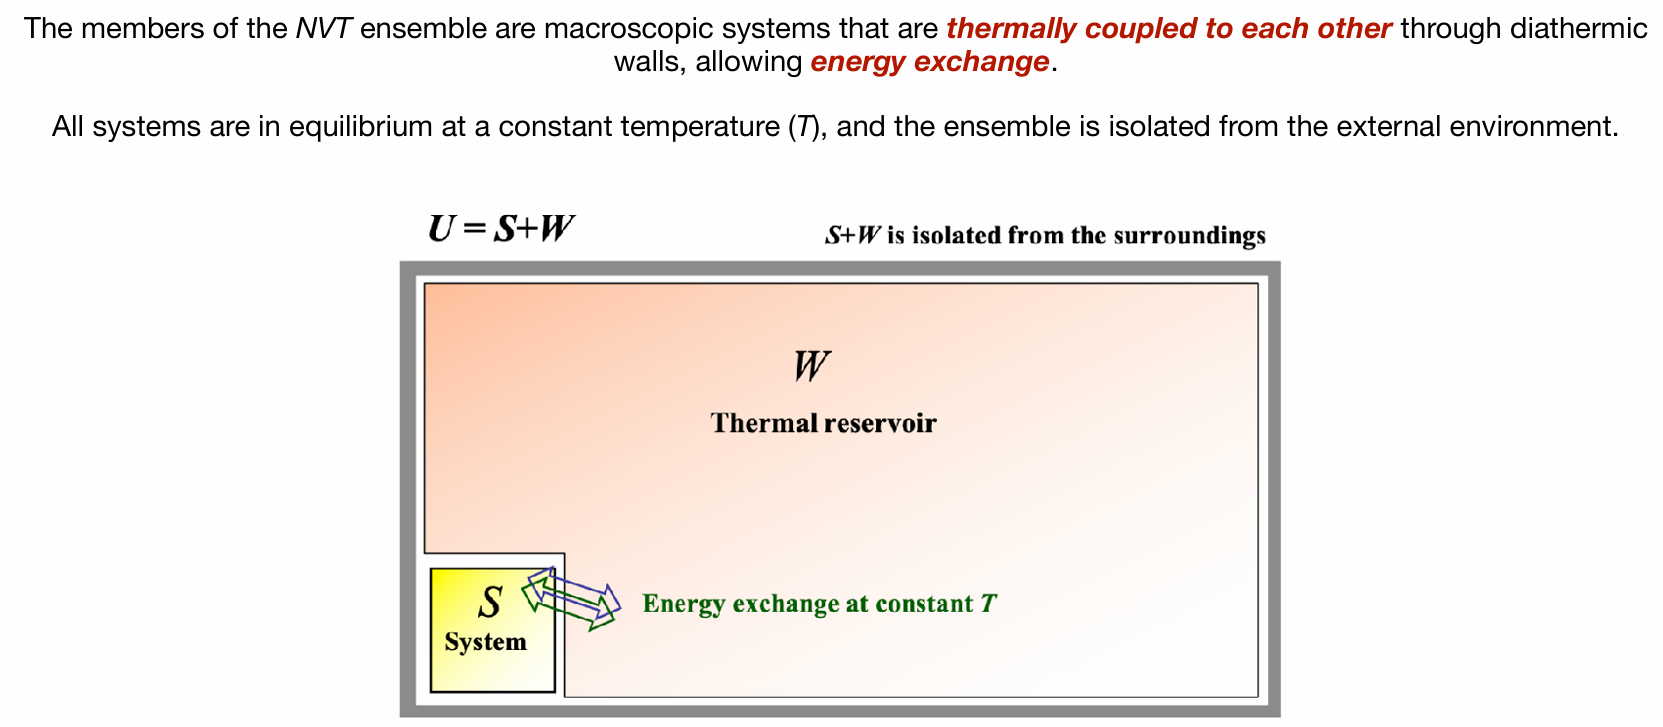
\includegraphics[width=0.7\textwidth]{IMG/canonical.png}
\end{figure}

\esp

In this chapter, we introduce and describe the \textbf{canonical ensemble}, also indicated as $NVT$ ensemble, which deals with systems that can exchange energy with a larger reservoir (bath) at a constant temperature. In the $NVT$ ensemble, systems are allowed to interact with an external reservoir, enabling energy exchanges.

\esp

This interaction permits the system to explore various energy states within the constraints of a fixed temperature. The resulting fluctuations among energy states contribute to the statistical distribution of energy across accessible states, allowing for a probabilistic description of the system.

\esp

The members of the $NVT$ ensemble are macroscopic systems thermally coupled through diathermic walls, allowing energy exchange between them. All systems are in equilibrium at a constant temperature ($T$), and the ensemble is isolated from the external surroundings as schematically illustrated in Fig. 5.1.

\subsection{Design of the Canonical Ensemble}

\begin{figure}[H]
	\centering
	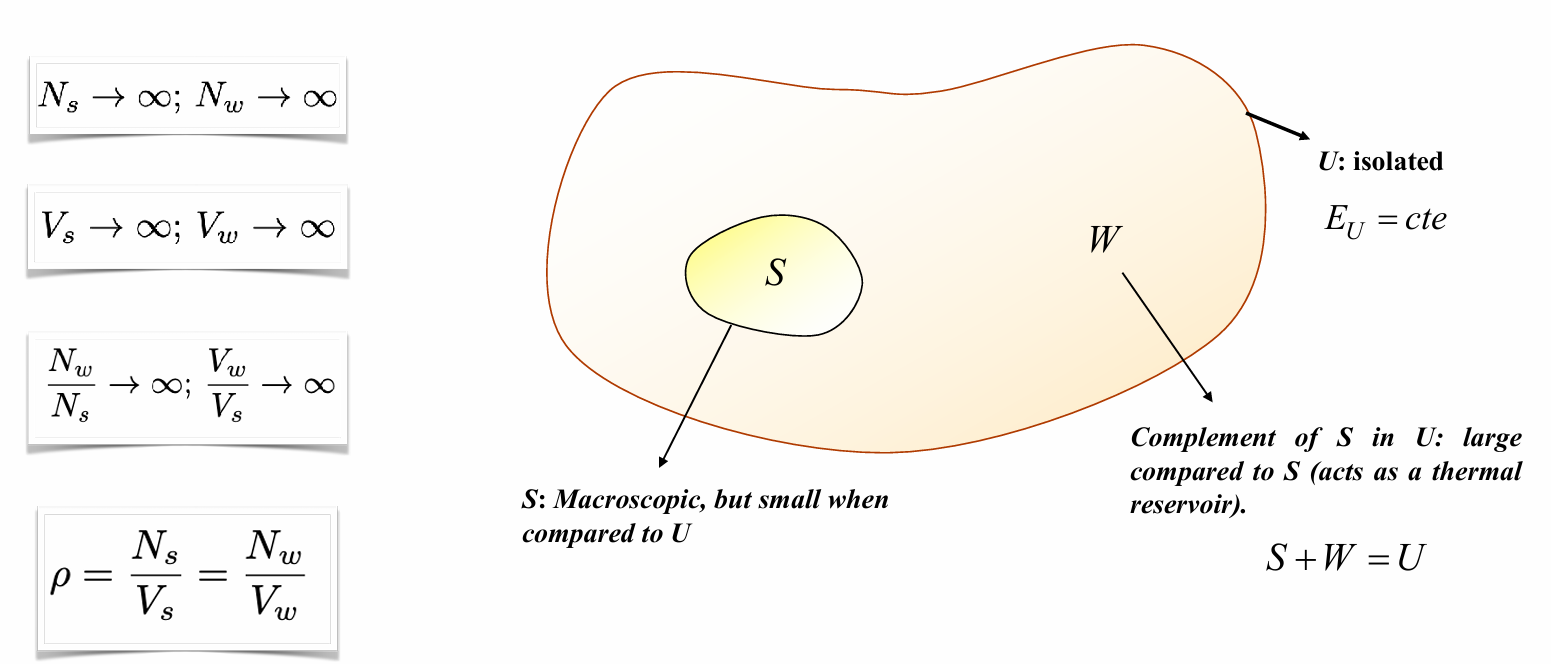
\includegraphics[width=0.7\textwidth]{IMG/design.png}
\end{figure}

With reference to Fig. 5.1, $U$ is an isolated \textit{supersystem} with $E_u$ constant. The system $S$ is a region of $U$ that is not strongly fluctuating and is macroscopic, but small compared to $U$. The complement of $S$ in $U$, indicated by $W$, is large compared to $S$ and acts as a thermal bath. We also know that $1 \ll N_s \ll N_w$, where $N_s$ and $N_w$ are, respectively, the number of particles in $S$ and in $W$. Similarly, $1 \ll V_s \ll V_w$, with $V_s$ and $V_w$ the volume occupied, respectively, by $S$ and $W$. In particular, the following relations hold:

\esp

\begin{equation}
	N_s \to \infty; N_w \to \infty; V_s \to \infty; V_w \to \infty \tag{5.1}
\end{equation}

\esp

and, in the thermodynamic limit, the size of the bath is infinitely larger than that of the system of interest. Mathematically, this condition is expressed as

\esp

\begin{equation}
	\frac{N_w}{N_s} \to \infty; \frac{V_w}{V_s} \to \infty \tag{5.2}
\end{equation}

\esp

We also assume that the density of $S$ equals the density of $W$:

\esp

\begin{equation}
	\rho = \frac{N_s}{V_s} = \frac{N_w}{V_w} \tag{5.3}
\end{equation}

\esp

\begin{figure}[H]
	\centering
	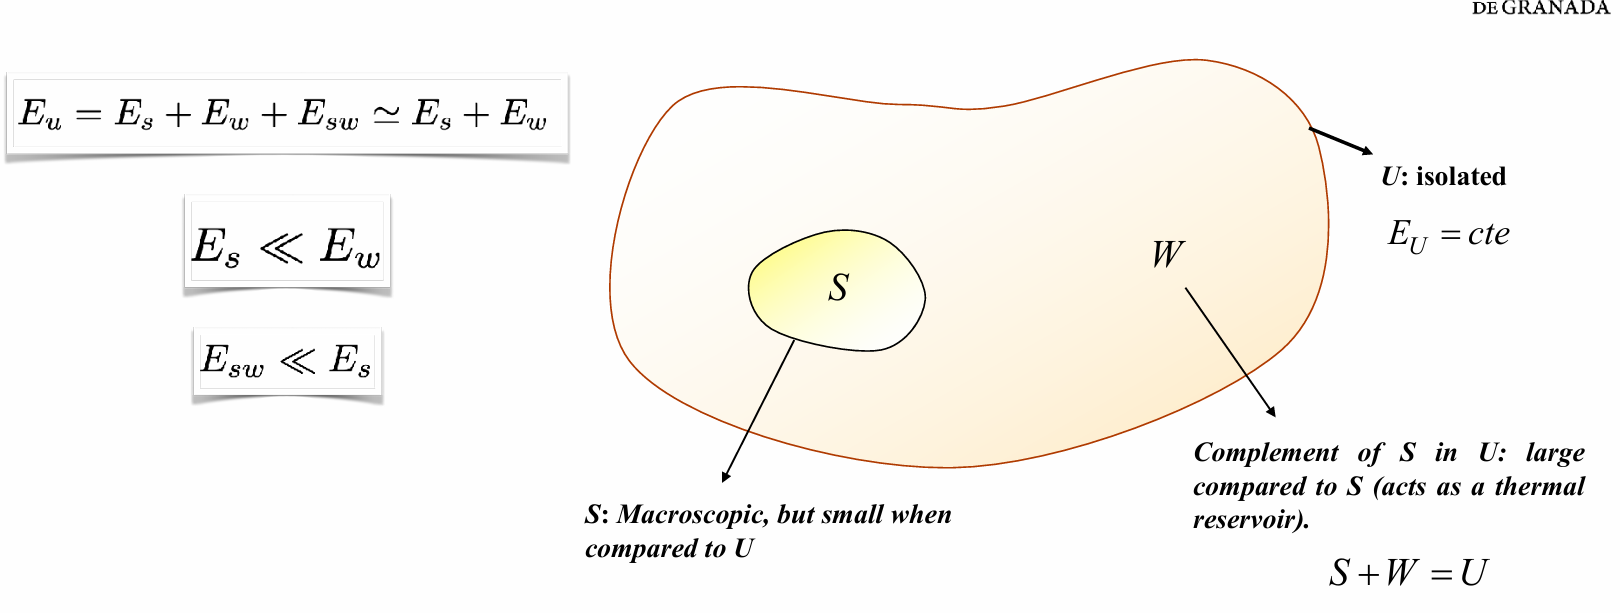
\includegraphics[width=0.7\textwidth]{IMG/design2.png}
\end{figure}

\esp

Finally, the internal energy of the supersystem (universe) is related to that of the system and the bath as follows:

\esp

\begin{equation}
	E_u = E_s + E_w + E_{sw} \simeq E_s + E_w \tag{5.4}
\end{equation}

\esp

\noindent where $E_s \ll E_w$ and $E_{sw} \ll E_s$ are negligible. As a consequence, given the negligible interaction between $S$ and $W$, one can write the following relation:

\esp

\begin{equation}
	E_m = E_m(N_s, V_s) \tag{5.5}
\end{equation}

\esp

\noindent where $E_m$, which depends on the number of particles and the volume of $S$, denotes the energy of an energy state $m$ in which $S$ can be found. If the energy of $S$ is $E_m$, then the energy of the thermal bath $W$ must lie between

\esp

\begin{equation}
	E_w = E_u - E_m \tag{5.6}
\end{equation}

\esp

\noindent and

\esp

\begin{equation}
	E_w + \Delta E. \tag{5.7}
\end{equation}

\esp

\noindent This energy interval of \textit{uncertainty} arises from the fact that energy cannot be measured exactly, as already noted in the discussion of the microcanonical ensemble in Chapter 4. From now on, to simplify the notation, we will use $N$ and $V$ to refer, respectively, to the number of particles and volume of $S$.

\subsubsection{Partition Function}

\begin{figure}[H]
	\centering
	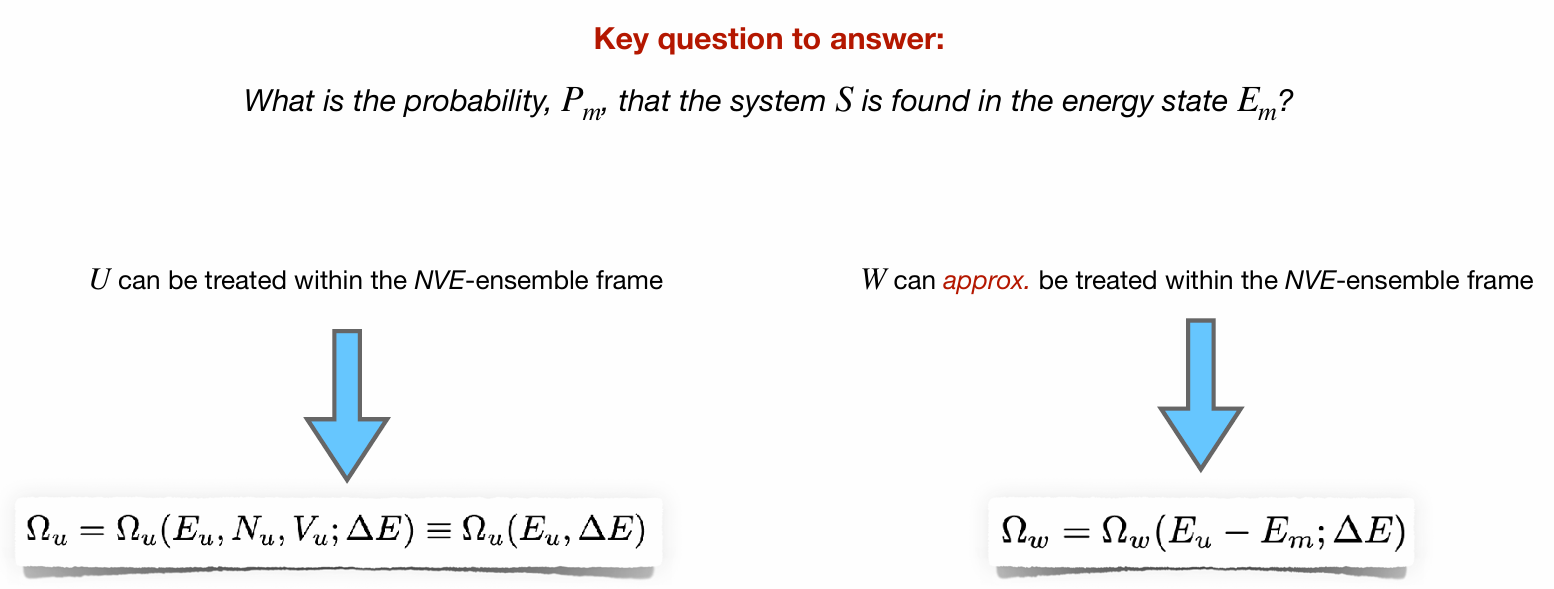
\includegraphics[width=0.7\textwidth]{IMG/partition.png}
\end{figure}

\esp

Now that the thermodynamic system of interest has been defined, the question we aim to address is: \textit{What is the probability, $P_m$, that the system $S$ is found in the energy state $E_m$?} To answer this question, we note that the supersystem $U$ is isolated, with $E_u, N_u,$ and $V_u$ constant. This implies that $U$ can be treated within the microcanonical ensemble framework. In particular,

\esp

\begin{equation}
	\Omega_u = \Omega_u(E_u, N_u, V_u; \Delta E) \equiv \Omega_u(E_u, \Delta E). \tag{5.8}
\end{equation}

\esp

Strictly speaking, the thermal bath $W$, with energy $E_u - E_m$, is not isolated, as it can exchange energy with $S$. Nevertheless, since $E_m \ll E_u$, we can neglect the effect of $S$ on $W$ and assume, to a good approximation, that $W$ is also effectively isolated:

\esp

\begin{equation}
	\Omega_w = \Omega_w(E_u - E_m; \Delta E). \tag{5.9}
\end{equation}

\esp

\begin{figure}[H]
	\centering
	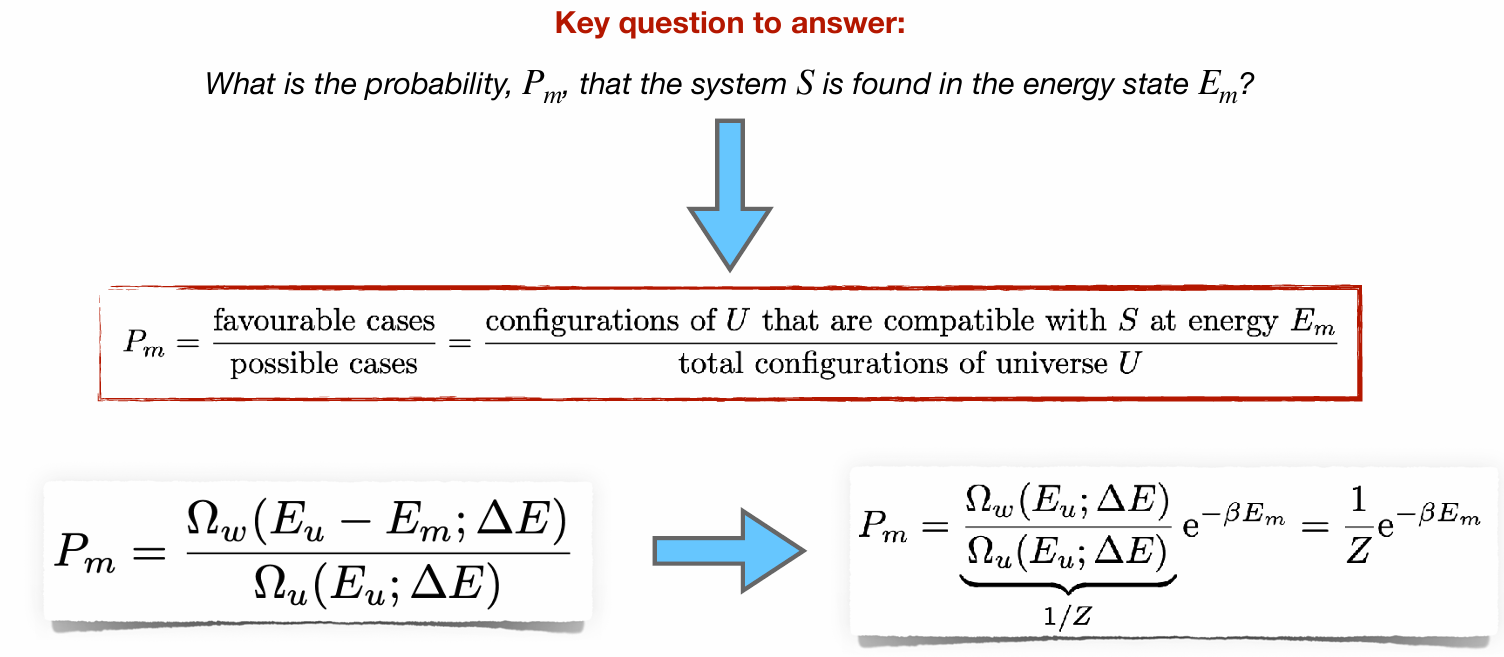
\includegraphics[width=0.7\textwidth]{IMG/partition2.png}
\end{figure}

We emphasize that $\Omega_w$ represents the number of configurations (states) in the universe $U$ that are compatible with an energy $E_m$ for $S$, where $E_w$ is such that the total energy falls within the range $[E_u, E_u + \Delta E]$. Additionally, since $W$ can be considered an isolated system (as its interactions with $S$ can be neglected), it can be treated within the microcanonical ensemble framework, implying that all its possible configurations (states) are equally probable. In light of these preliminary considerations, let's calculate this probability:

\esp

\begin{equation}
	P_m = \frac{\text{favourable cases}}{\text{possible cases}} = \frac{\text{configurations of } U \text{ that are compatible with } S \text{ at energy } E_m}{\text{total configurations of universe } U} \tag{5.10}
\end{equation}

\esp

equivalently

\esp

\begin{equation}
	P_m = \frac{\Omega_w(E_u - E_m; \Delta E)}{\Omega_u(E_u; \Delta E)} \tag{5.11}
\end{equation}

\esp

Given that $E_m \ll E_u$, we can develop a power series of $\Omega_w$. However, since $\Omega$ is generally a function that increases exponentially with energy, the convergence of the series will be very slow. An alternative is expanding $\ln \Omega_w$:

\esp

\begin{equation}
	\ln \Omega_w(E_w; \Delta E) = \ln \Omega_w(E_u; \Delta E) + \underbrace{\left( \frac{\partial \ln \Omega_w}{\partial E} \right)_{E=E_u}}_{\beta} (E_w - E_u) + \dots \simeq \ln \Omega_w(E_u; \Delta E) - \beta E_m \tag{5.12}
\end{equation}

\esp

Rearranging, we obtain

\esp

\begin{equation}
	\Omega_w(E_u - E_m; \Delta E) \simeq \Omega_w(E_u; \Delta E) e^{-\beta E_m} \tag{5.13}
\end{equation}

\esp

and substituting in Eq. 6.20, we get

\esp

\begin{equation}
	P_m = \underbrace{\frac{\Omega_w(E_u; \Delta E)}{\Omega_u(E_u; \Delta E)}}_{1/Z} e^{-\beta E_m} = \frac{1}{Z} e^{-\beta E_m} \tag{5.14}
\end{equation}

\esp

where $Z$ is the \textbf{canonical partition function}. The best way to calculate $Z$ is not to use Eq. 5.14, but to recall the normalisation condition of probability:

\esp

\begin{equation}
	\sum_m P_m = \sum_m \frac{1}{Z} e^{-\beta E_m} = \frac{1}{Z} \sum_m e^{-\beta E_m} = 1 \tag{5.15}
\end{equation}

\esp

It follows that

\esp

\begin{equation}
	Z = \sum_m e^{-\beta E_m} \tag{5.16}
\end{equation}

\esp

and equivalently

\esp

\begin{equation}
	Z = \sum_n \Omega(E_n) e^{-\beta E_n} \tag{5.17}
\end{equation}

\esp

where $n$ indicates the number of energy levels. Since each energy level $E_n$ can have multiple states associated with it, $Z$ can be expressed either as a sum over individual states or as a sum over energy levels weighted by their degeneracy $\Omega(E_n)$, as in Eq. 5.17. The partition function $Z$ encodes how the probabilities are \textbf{partitioned} among the different states, based on their individual energies$^1$. It represents the sum over all the energy states of $S$ compatible with the same $NVT$-macrostate or, equivalently, the sum over all the energy levels observed in $S$. The partition function is much easier to calculate than $\Omega$ and is valid for systems that are more general than the isolated one.

\esp

\begin{figure}[H]
	\centering
	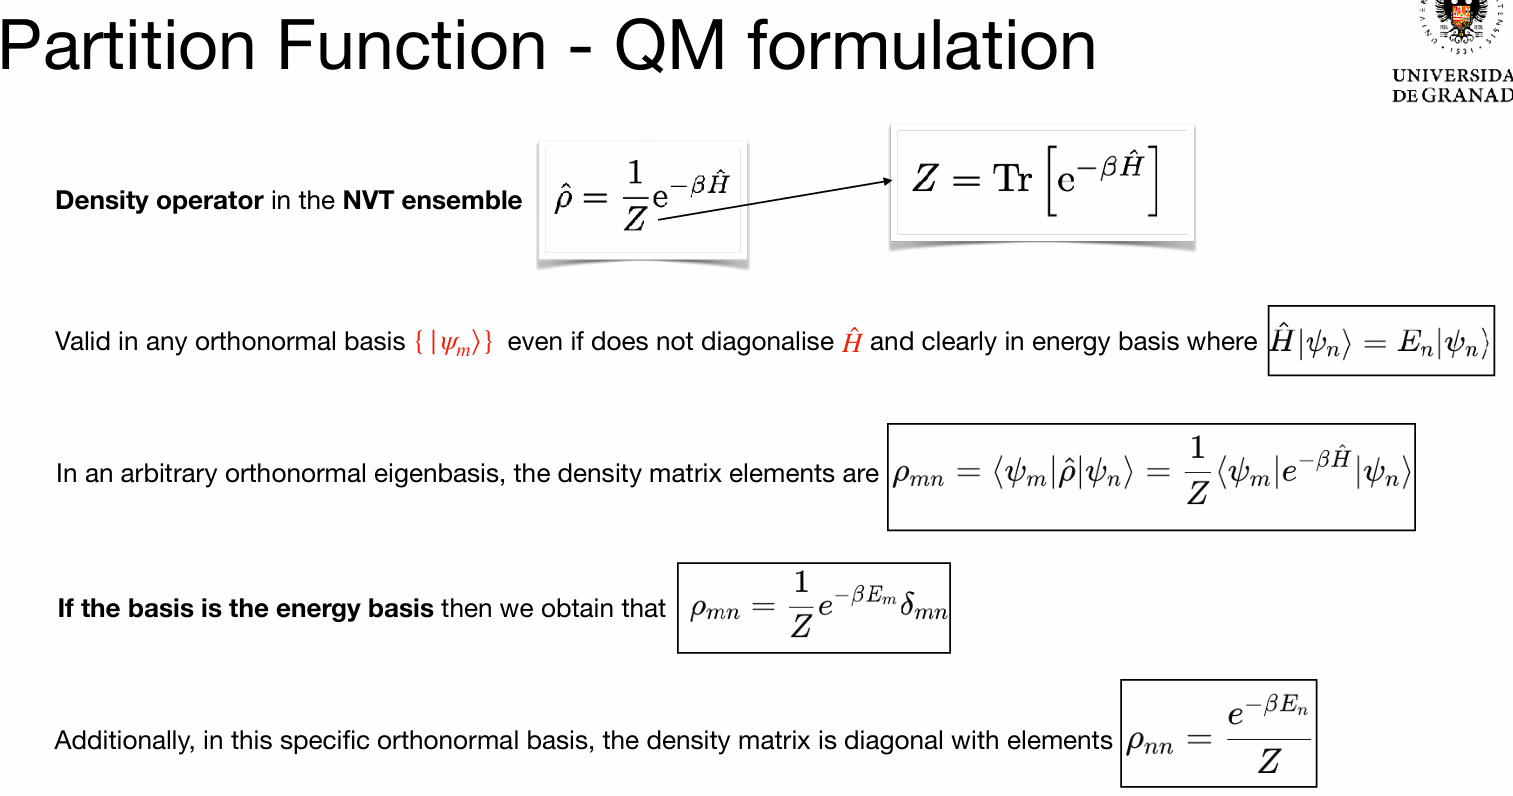
\includegraphics[width=0.7\textwidth]{IMG/partitionqp.png}
\end{figure}

\esp

The quantum formulation of the canonical ensemble is represented by the density matrix $\rho_{mn}$, which is given by:

\esp

\begin{equation}
	\rho_{mn} = \frac{1}{Z} e^{-\beta E_m} \delta_{mn} . \tag{5.18}
\end{equation}

\esp

In general, expectation values are calculated as

\esp

\begin{equation}
	\langle B \rangle = \sum_{m} P_m B_m = \frac{1}{Z} \sum_{m} B_m e^{-\beta E_m} , \tag{5.19}
\end{equation}

\esp

where $B_m = \langle \phi_m | \hat{B} | \phi_m \rangle$ is the expectation value of $\hat{B}$ in the eigenstate $|\phi_m\rangle$. One of the key advantages of the canonical ensemble is that it can be applied using any orthonormal basis $|\psi_m\rangle$, even if it does not diagonalize $\hat{H}$. This implies that solving Schrödinger's equation explicitly is not necessary. In terms of the density operator, we define:

\esp

\begin{equation}
	\hat{\rho} = \frac{1}{Z} e^{-\beta \hat{H}} . \tag{5.20}
\end{equation}

\esp

\begin{figure}[H]
	\centering
	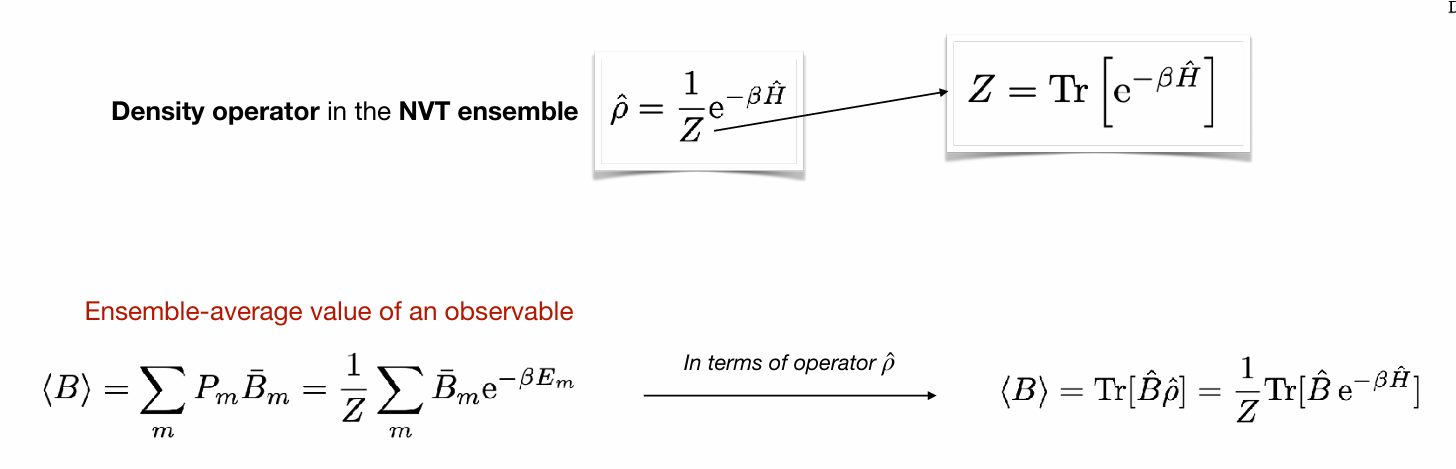
\includegraphics[width=0.7\textwidth]{IMG/partitionqp2.png}
\end{figure}

\esp

\noindent It follows that

\esp

\begin{equation}
	\langle B \rangle = \text{Tr}[\hat{B}\hat{\rho}] = \frac{1}{Z} \text{Tr} \left[ \hat{B} e^{-\beta \hat{H}} \right] . \tag{5.21}
\end{equation}

\esp

Thus, we can use any orthonormal basis of the Hilbert space to perform numerical calculations:

\esp

\begin{equation}
	Z = \text{Tr} \left[ e^{-\beta \hat{H}} \right] . \tag{5.22}
\end{equation}

\esp

\section{Connection with Thermodynamics}

\begin{figure}[H]
	\centering
	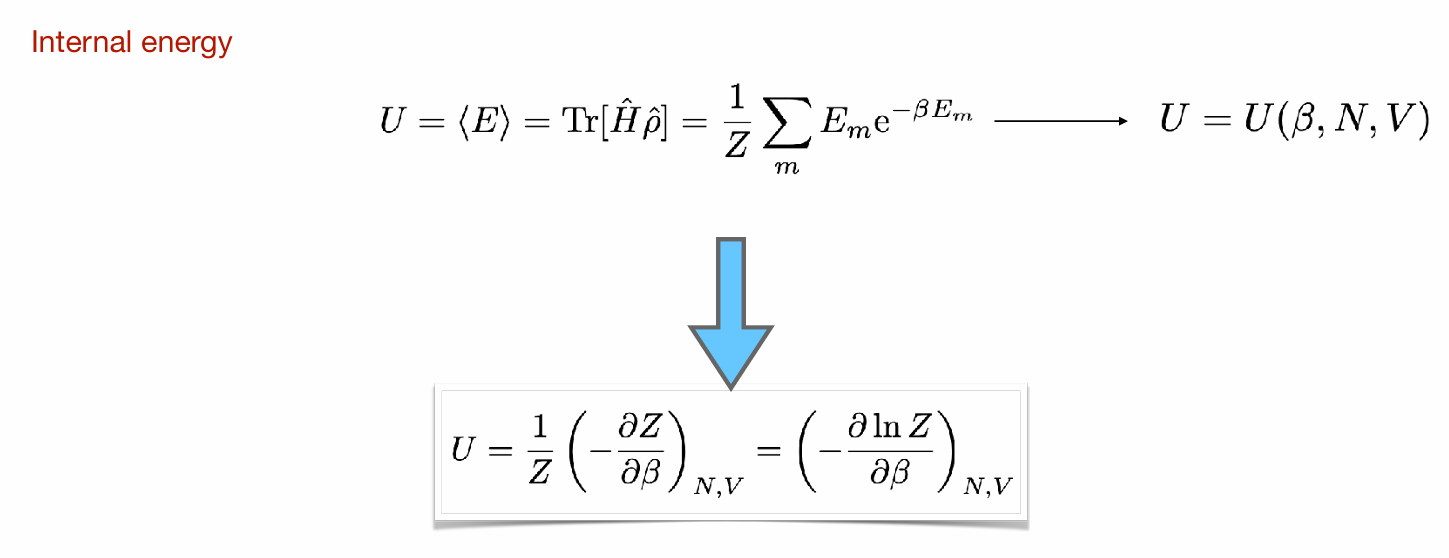
\includegraphics[width=0.7\textwidth]{IMG/thermo.png}
\end{figure}

\esp

Thermodynamics begins with a few empirical observations, which are organised and axiomatised in the form of four laws. From these laws, thermodynamics establishes relationships between several properties that characterise the thermal behaviour of a macroscopic system. However, thermodynamics presents an important drawback: \textbf{it does not allow the calculation of absolute values for any property}. For example, if we know $C_V$, we can determine $C_P$ and viceversa; thermodynamics provides the relationship between them but not their specific values. Statistical Physics can resolve this inconvenience; specifically, the canonical ensemble provides a model for thermal equilibrium. More specifically, Statistical Physics is capable of obtaining thermodynamic (macroscopic) properties in terms of microscopic magnitudes of molecules. In the case of the canonical ensemble, if we know the energy spectrum $\{E_n\}$, we can deduce the thermodynamic variables. Similarly, Statistical Physics allows for the calculation of microscopic properties from macroscopic observations (for example, intermolecular interactions).

\esp

Thermodynamic variables can be classified into three groups:

\esp

\begin{itemize}
	\item \textbf{External Parameters}, such as $N$ (number of particles), $V$ (volume), etc. Fixed by the experimenter or the system's environment.
	\item \textbf{Mechanical Properties}, such as $p$ (pressure), $U$ (internal energy), etc. They are averages of microscopic dynamic functions.
	\item \textbf{Thermal Properties}, such as $T$ (temperature), $S$ (entropy). They do not have a microscopic equivalent (at the particle level). They can only be defined at the macroscopic level. They are collective properties whose value is determined by the entire ensemble.
\end{itemize}

\esp

The first connection is provided by the internal energy:

\esp

\begin{equation}
	U = \langle E \rangle = \text{Tr}[\hat{H}\hat{\rho}] = \frac{1}{Z} \sum_{m} E_m e^{-\beta E_m} \tag{5.23}
\end{equation}

\esp

We note that $U = U(\beta, N, V)$, although we still have to see what $\beta$ is. Now, since the system can exchange energy with the environment (in equilibrium), $E$ is no longer fixed but can fluctuate. The internal energy is its mean value $U = \langle E \rangle$. It is possible to re-write Eq. 6.28 in a more practical fashion:

\esp

\begin{equation}
	U = \sum_{m} E_m P_m = \frac{1}{Z} \sum_{m} E_m e^{-\beta E_m} = \frac{1}{Z} \sum_{m} \left( -\frac{\partial}{\partial \beta} e^{-\beta E_m} \right) = \frac{1}{Z} \left( -\frac{\partial}{\partial \beta} \right) \sum_{m} e^{-\beta E_m} \tag{5.24}
\end{equation}

\esp

Equivalently:

\esp

\begin{equation}
	U = \frac{1}{Z} \left( -\frac{\partial Z}{\partial \beta} \right)_{N,V} = -\left( \frac{\partial \ln Z}{\partial \beta} \right)_{N,V} \tag{5.25}
\end{equation}

\esp

To find out further connections with Thermodynamics, specifically that $\beta$ is closely related to the temperature, we now consider the configuration given in Fig. 5.2.

\esp

\begin{figure}[H]
	\centering
	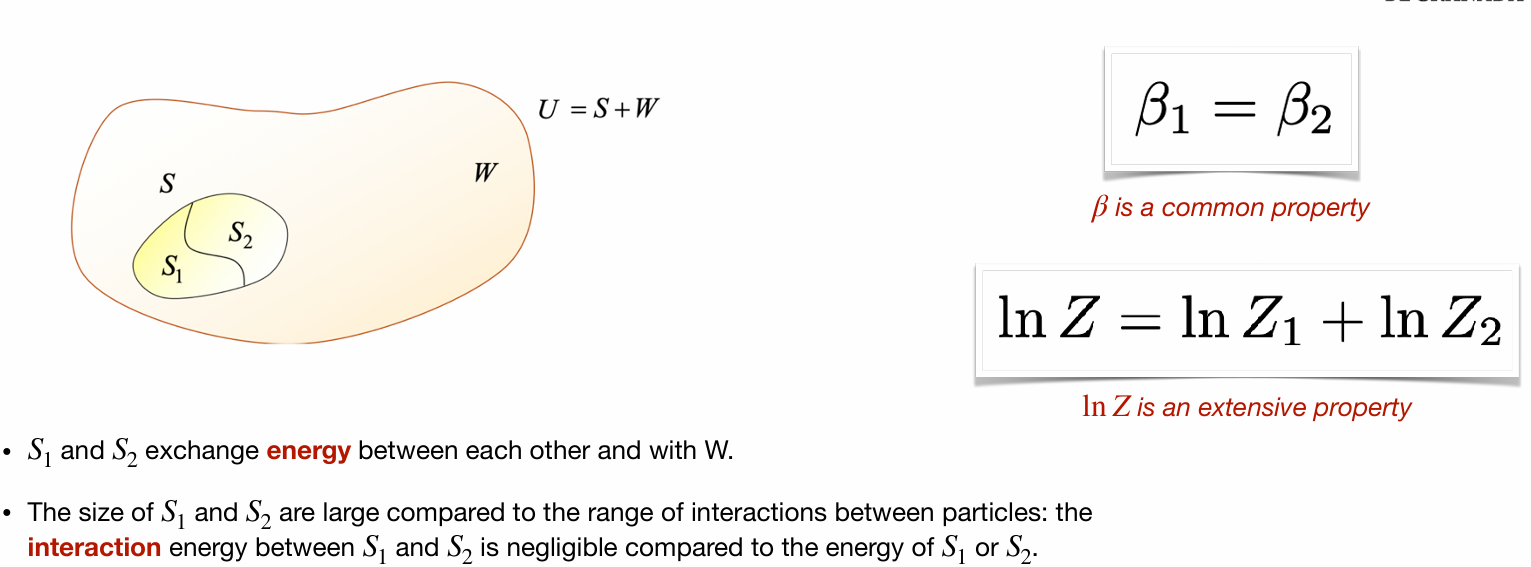
\includegraphics[width=0.7\textwidth]{IMG/thermo2.png}
\end{figure}

\esp

Systems $S_1$ and $S_2$ exchange energy between themselves and with $W$ and the three systems are at thermal equilibrium with each other. We will assume that the sizes of $S_1$ and $S_2$ are large compared to the range of interactions between particles: the interaction energy between $S_1$ and $S_2$, although physically significant in ensuring the exchange of energy, is negligible compared to the energy of $S_1$ or $S_2$. What is the probability, $P_{n,m}$, of finding system $S_1$ in the energy state $E_{1n}$ and $S_2$ in $E_{2m}$? To answer this question, we have two options:

\esp

\begin{itemize}
	\item If we consider $S$ as a sum of $S_1$ and $S_2$, then
	\begin{equation}
		P_{n,m} = P_n^{(1)} P_m^{(2)} = \frac{1}{Z_1} e^{-\beta_1 E_{1,n}} \frac{1}{Z_2} e^{-\beta_2 E_{2,m}} \tag{5.26}
	\end{equation}
	This is basically the product of two independent probabilities, with, in principle, $\beta_1 \neq \beta_2$.
	
	\esp
	
	\item If we can look at $S$ as a unique system, then
	\begin{equation}
		P_{n,m} = \frac{1}{Z} e^{-\beta(E_{1,n} + E_{2,m})} \tag{5.27}
	\end{equation}
\end{itemize}

\esp

The probability $P_{n,m}$ must be the same regardless the option applied. This implies that

\esp

\begin{equation}
	\frac{1}{Z_1 Z_2} e^{-\beta_1 E_{1,n}} e^{-\beta_2 E_{2,m}} = \frac{1}{Z} e^{-\beta(E_{1,n} + E_{2,m})} \tag{5.28}
\end{equation}

\esp

Since this equation is true $\forall E_{1,n}$ and $\forall E_{2,m}$, then it follows that

\esp

\begin{equation}
	\beta_1 = \beta_2 \tag{5.29}
\end{equation}

\esp

Because thermodynamics asserts that two systems in equilibrium must have the same temperature, it must be that

\esp

is an \textbf{intensive} property (in particular, $\beta = 1/kT$). We also see that

\esp

\begin{equation}
	Z = Z_1 Z_2 \tag{5.31}
\end{equation}

\esp

which implies that

\esp

\begin{equation}
	\ln Z = \ln Z_1 + \ln Z_2 \tag{5.32}
\end{equation}

\esp

is an additive or \textbf{extensive} property. Moreover, we see that $\beta$ \textbf{is a common property}, being the same in all systems when thermal equilibrium is achieved. 

\esp

\begin{figure}[H]
	\centering
	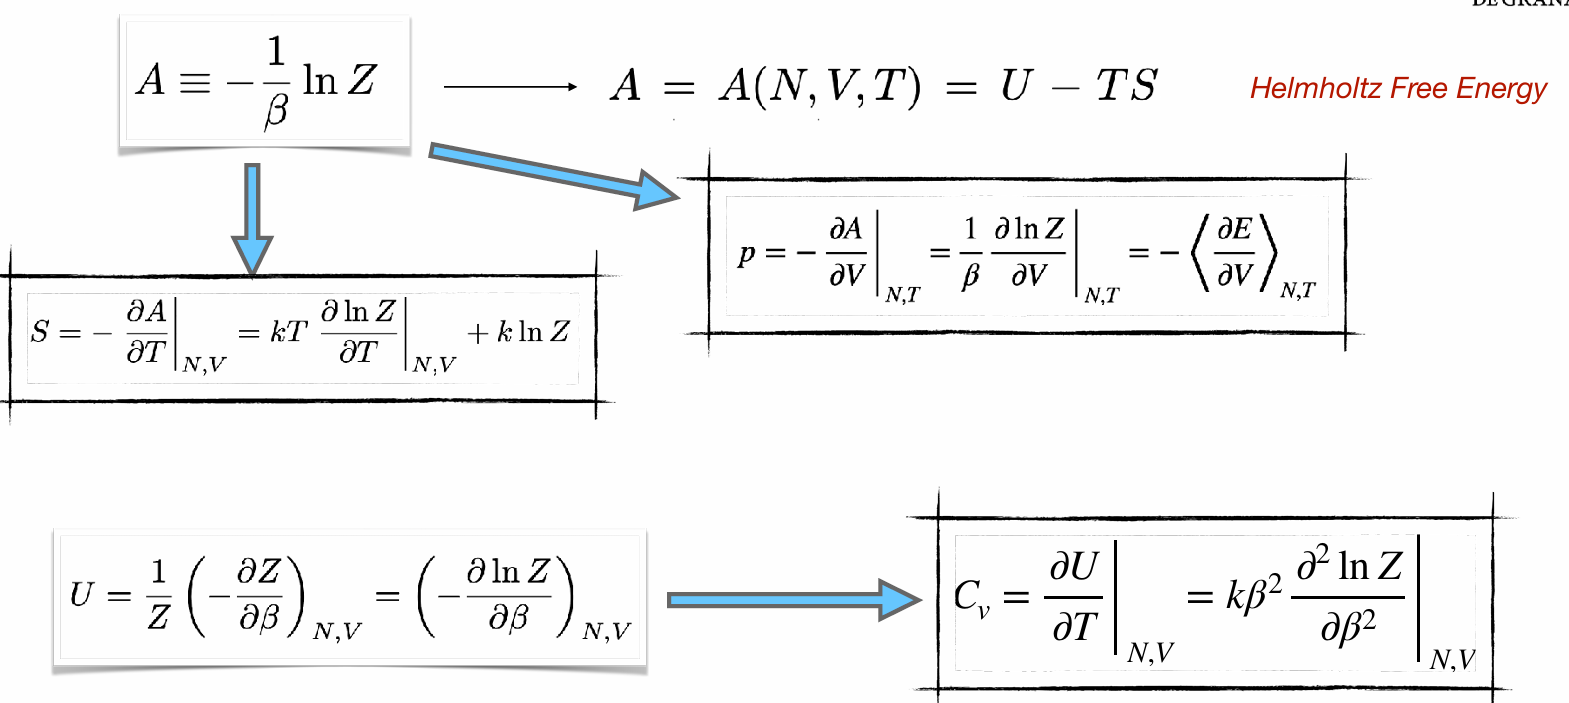
\includegraphics[width=0.7\textwidth]{IMG/thermo3.png}
\end{figure}

\esp

By applying these two conclusions, we can define the following function

\esp

\begin{equation}
	A \equiv -\frac{1}{\beta} \ln Z \tag{5.33}
\end{equation}

\esp

which is also extensive as $A_{1+2} = A_1 + A_2$. What does $A$ represent? To find that out, let's calculate the total derivative of $\beta A$, noting that $A = A(\beta, \{E_n\})$

\esp

\begin{equation}
	d(\beta A) = \left. \frac{\partial(\beta A)}{\partial \beta} \right|_{\{E_n\}} d\beta + \sum_{n} \left. \frac{\partial(\beta A)}{\partial E_n} \right|_{\beta} dE_n \tag{5.34}
\end{equation}

\esp

The first term in the right hand side of the above equation is equal to the internal energy (see also Eq. 5.25):

\esp

\begin{equation}
	\left. \frac{\partial(\beta A)}{\partial \beta} \right|_{\{E_n\}} = -\left. \frac{\partial(\ln Z)}{\partial \beta} \right|_{\{E_n\}} = -\left. \frac{\partial(\ln Z)}{\partial \beta} \right|_{N,V} = U \tag{5.35}
\end{equation}

\esp

The second term is a probability. Let's see why:

\esp

\begin{equation}
	\left. \frac{\partial(\beta A)}{\partial E_n} \right|_{\beta} = -\left. \frac{\partial(\ln Z)}{\partial E_n} \right|_{\beta} = -\frac{1}{Z} \left. \frac{\partial Z}{\partial E_n} \right|_{\beta} = -\frac{1}{Z} \frac{\partial}{\partial E_n} \left( \sum_{m} e^{-\beta E_m} \right)_{\beta} = \beta \frac{e^{-\beta E_n}}{Z} = \beta P_n \tag{5.36}
\end{equation}

\esp

Substituting these results in Eq. 5.34, we obtain

\esp

\begin{equation}
	d(\beta A) = U d\beta + \beta \sum_{n} P_n dE_n \tag{5.37}
\end{equation}

\esp

Since $U d\beta = d(\beta U) - \beta dU$, we can rewrite this equation as

\esp

\begin{equation}
	d[\beta(U - A)] = \beta dU - \beta \sum_{n} P_n dE_n \tag{5.38}
\end{equation}

\esp

We have now to understand what the summation in the above equation, that is $\sum_{n} P_n dE_n$, represents \textit{thermodynamically}. To this end, we first note that $dE_n$ is an energy change of the system following an \textbf{adiabatic volume change}$^2$. Mathematically, this volume-driven energy change can be expressed as

\esp

\begin{equation}
	E_n' = E_n + \left. \frac{\partial E_n}{\partial V} \right|_{N} dV \tag{5.39}
\end{equation}

\esp

Therefore

\esp

\begin{equation}
	\sum_{n} P_n dE_n = \underbrace{\sum_{n} P_n E_n'}_{U'} - \underbrace{\sum_{n} P_n E_n}_{U} = dU_{\text{adiabatic}} \tag{5.40}
\end{equation}

\esp

The First Law of Thermodynamics (conservation of energy) states that $dU = đQ + đW$, where $đQ$ and $đW$ represent, respectively, the amount of heat and work exchanged between the system and its surroundings$^3$. Because the process we are considering is adiabatic, the First Law reduces to $dU_{\text{adiabatic}} = đW$. In particular,

\esp

\begin{equation}
	dU_{\text{adiabatic}} = đW = \sum_{n} P_n dE_n = \sum_{n} P_n \left. \frac{\partial E_n}{\partial V} \right|_N dV \tag{5.43}
\end{equation}

\esp

Since the work exchanged as a result of a volume change is $đW = -pdV$, we can rewrite the last equation as

\esp

\begin{equation}
	\sum_{n} P_n \left. \frac{\partial E_n}{\partial V} \right|_N dV = -pdV \tag{5.44}
\end{equation}

\esp

Rearranging, we obtain an expression for pressure:

\esp

\begin{equation}
	p = -\sum_{n} P_n \left. \frac{\partial E_n}{\partial V} \right|_N \tag{5.45}
\end{equation}

\esp

If we now substitute this result into Eq. 5.38, we get

\esp

\begin{equation}
	d[\beta(U - A)] = \beta dU - \beta \sum_{n} P_n dE_n = \beta[dU - đW] = \beta đQ \tag{5.46}
\end{equation}

\esp

It is interesting and useful to observe that, by multiplying $đQ$ by $\beta$, one can transform this inexact differential into the exact differential $d[\beta(U - A)]$. This implies that $\beta$ is the \textit{integrating factor} of $đQ^4$. If we now apply the Second Law of Thermodynamics $đQ = TdS$, we obtain

\esp

\begin{equation}
	d[\beta(U - A)] = \beta đQ = \beta TdS \tag{5.47}
\end{equation}

\esp

This implies that the property $A = A(N,V,T) = U - TS$, defined in Eq. 5.33, is the \textbf{Helmholtz free energy}. The total differential of $A(N,V,T)$ reads

\esp

\begin{equation}
	dA = \left. \frac{\partial A}{\partial N} \right|_{V,T} dN + \left. \frac{\partial A}{\partial V} \right|_{N,T} dV + \left. \frac{\partial A}{\partial T} \right|_{N,V} dT = -d \left( \frac{1}{\beta} \ln Z \right) . \tag{5.48}
\end{equation}

\esp

It follows that

\esp

\begin{align}
	\mu &= \left. \frac{\partial A}{\partial N} \right|_{V,T} = \frac{1}{Z} \sum_{m} \left( \left. \frac{\partial E_m}{\partial N} \right|_{V,T} e^{-\beta E_m} \right) = \left\langle \frac{\partial E}{\partial N} \right\rangle_{V,T} \tag{5.49} \\
	\esp
	p &= -\left. \frac{\partial A}{\partial V} \right|_{N,T} = \frac{1}{\beta} \left. \frac{\partial \ln Z}{\partial V} \right|_{N,T} = -\frac{1}{Z} \sum_{m} \left( \left. \frac{\partial E_m}{\partial V} \right|_{N,T} e^{-\beta E_m} \right) = -\left\langle \frac{\partial E}{\partial V} \right\rangle_{N,T} \tag{5.50} \\
	\esp
	S &= -\left. \frac{\partial A}{\partial T} \right|_{N,V} = kT \left. \frac{\partial \ln Z}{\partial T} \right|_{N,V} + k \ln Z = k(\beta \langle E \rangle + \ln Z) \tag{5.51}
\end{align}

\esp

We already know the expression of the internal energy $U = -\left. \frac{\partial \ln Z}{\partial \beta} \right|_{N,V}$, from which the heat capacity at constant volume is obtained:

\esp

\begin{equation}
	C_v = \left. \frac{\partial U}{\partial T} \right|_{N,V} = \left. \frac{\partial U}{\partial \beta} \frac{\partial \beta}{\partial T} \right|_{N,V} = \frac{1}{kT^2} \left. \frac{\partial^2 \ln Z}{\partial \beta^2} \right|_{N,V} = k \beta^2 \left. \frac{\partial^2 \ln Z}{\partial \beta^2} \right|_{N,V} \tag{5.52}
\end{equation}

\esp

We can also express entropy in terms of probability only. Let's start with the operative definition of probability:

\esp

\begin{equation}
	P_n = \frac{e^{-\beta E_n}}{Z} \iff \ln P_n = -\beta E_n - \ln Z \tag{5.53}
\end{equation}

\esp

We can use $P_n$ to determine the average value of energy:

\esp

\begin{equation}
	\beta \langle E \rangle = \sum_n P_n \beta E_n = \sum_n P_n (-\ln P_n - \ln Z) = -\sum_n P_n \ln P_n - \ln Z \sum_n P_n = -\sum_n P_n \ln P_n - \ln Z \tag{5.54}
\end{equation}

\esp

Therefore

\esp

\begin{equation}
	S = k(\beta \langle E \rangle + \ln Z) = k \left( -\sum_n P_n \ln P_n - \cancel{\ln Z} + \cancel{\ln Z} \right) = -k \sum_n P_n \ln P_n \tag{5.55}
\end{equation}

\esp

We see that entropy depends solely on the probability values: it does not possess any associated microscopic magnitude; it is a \textbf{thermal quantity}. Eq. 5.55 leads to several important conclusions:

\esp

\begin{itemize}
	\item If the system is in the ground state (at $T = 0$ K), and this state is unique, then $P_n = 1$ for this state and zero for all other states. The value of entropy for this state is zero, which is essentially the \textbf{Third Law of Thermodynamics}.
	\item As the temperature increases, the number of accessible energy states increases, and the values of $P_n$ above the ground level are no longer zero. This leads to an increase in entropy. \textbf{Higher entropy implies a higher degree of statistical disorder within the system.}
\end{itemize}

\esp

Finally, we can express the partition function in terms of states or energy levels:

\esp

\begin{equation}
	Z = \underbrace{\sum_m}_{\text{states}} e^{-\beta E_m} = \underbrace{\sum_n}_{\text{energy levels}} \sum_{[j]_n} e^{-\beta E_n} = \sum_n e^{-\beta E_n} \sum_{[j]_n} 1 = \sum_n \Omega(E_n) e^{-\beta E_n} \tag{5.56}
\end{equation}

\esp

where $[j]_n$ indicates the number of states with energy level compatible with $n$. We also remember that

\esp

\begin{equation}
	P_m = \frac{1}{Z} e^{-\beta E_m} \tag{5.57}
\end{equation}

\esp

and

\esp

\begin{equation}
	\langle B \rangle = \frac{1}{Z} \sum_m B_m e^{-\beta E_m} \tag{5.58}
\end{equation}

\begin{figure}[H]
	\centering
	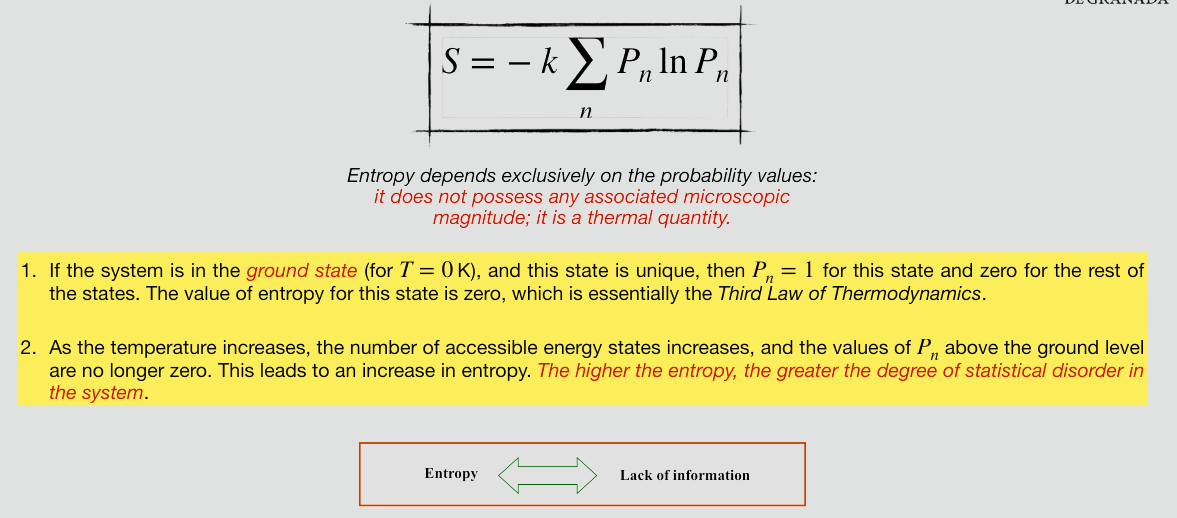
\includegraphics[width=0.7\textwidth]{IMG/thermo4.png}
\end{figure}

\section{Partition Function. Classical and Quantum Formalism}

\begin{figure}[H]
	\centering
	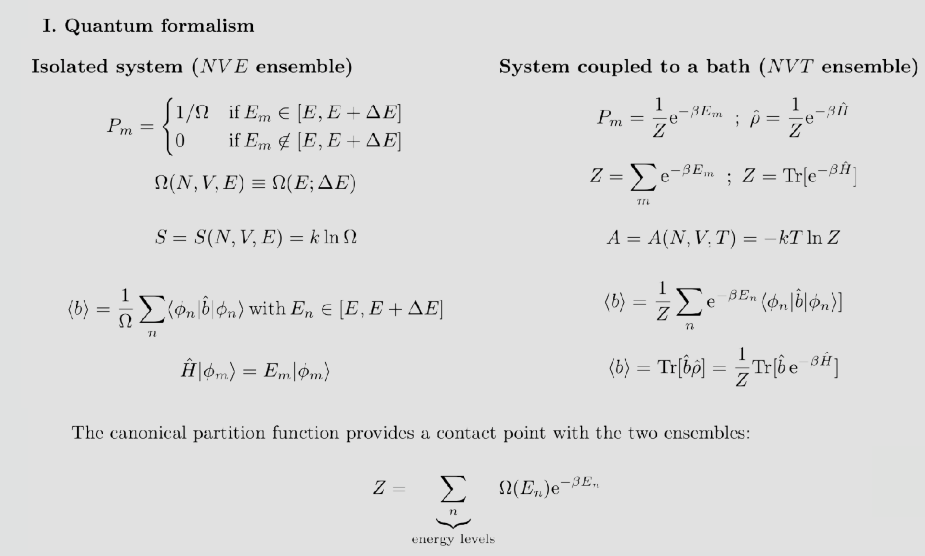
\includegraphics[width=0.7\textwidth]{IMG/versus.png}
\end{figure}

\esp

\begin{figure}[H]
	\centering
	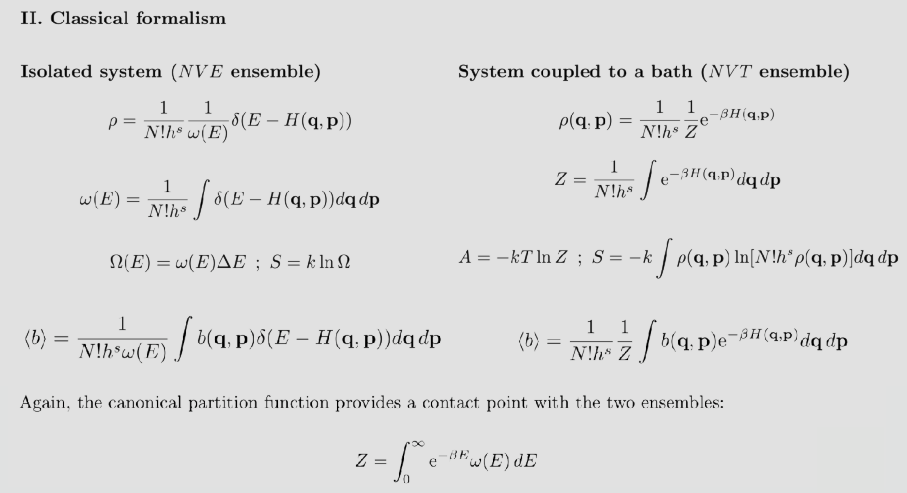
\includegraphics[width=0.7\textwidth]{IMG/versus2.png}
\end{figure}

\esp

\noindent \textbf{SOME PROVES IN RAW}

\printbibliography[title={Bibliografía}]
\end{document}